\newpage
\section{Sztuczna inteligencja w rolnictwie}
Metody sztucznej inteligencji(z ang. Artificial Inteligence - AI) znajdują szerokie zastosowanie w przemyśle rolniczym. Przemysł rolniczy, jako jedna z najważniejszych gałęzi światowej gospodarki, aktywnie rozwija się w celu optymalizacji produkcji żywności, wykorzystując w tym celu, między innymi sztuczną inteligencje. Sztuczna inteligencja znajduję zastosowanie w wielu aspektach prowadzenia działalności rolniczej. AI jest wykorzystywane do prognozowania i szacowania wielkości plonów. Na podstawie zdjęć modele są wstanie określić ilość plonów zdatnych do zebrania. Niektóre takie rozwiązania są wstanie określić, czy owoce na danym krzaku są zdatne do spożycia i zainicjować proces zbierania. Niektóre rozwiązania zbierają dane z pól i tworzą raport dla rolnika na temat dojrzałości zbiorów, co pozwala mu na lepsze zaplanowanie sezonu. Inne rozwiązania wykorzystują dane pogodowe, aby określić stopień dojrzałości upraw. SI wykorzystywane jest także w ramach klasyfikacji zdjęć. Istnieje wiele rozwiązań, które dokonują detekcji chorób roślin na podstawie np. zdjęć liści i ich diagnozy. Klasyfikacja stosowana jest też w detekcji chwastów i szkodników. SI wykorzystywana jest także w ocenie jakości plonów. Znajduje także zastosowanie w zarządzaniu chowem, gdzie na podstawie np. zachowań krów dokonuje klasyfikacji ich zachowania. Istnieją także rozwiązania, które pozwalają zaoszczedzić wodę - modele na podstawie danych ze szklarni, np. wilgotność ziemii dokonuje decyzji, czy należy podlać rosliny. Sztuczna inteligencja więc, nie tylko pozwala na zoptymalizowanie procesu produkcji żywności pochodzenia roślinnego, czy zwierzęcego, lecz pozwala także na oszczędzanie zasobów takich jak woda, co w czasach globalnego ocieplenia oraz susz, szczególnie w Polsce, staje się zasobem, który należy oszczędzać. \cite{liakos2018mlagriculture}
\subsection{Przykłady aplikacji}
Poniżej przedstawione aplikacje to rozwiązania ogólno dostępne w sklepie Play, wykorzystujące klasyfikacje z pomocą sztucznej inteligencji w celu identyfikacji roślin, bądź także identyfikacji trapiących ich chorób. Są one przykładem praktycznego zastosowania technologii klasyfikacji w codziennym życiu.
\subsubsection{Planta: Plant \& Garden Care}
Aplikacja skierowana do osób zajmujących się hodowlą roślin. W aplikacji znajduje się atlas roślin, w którym znajdziemy informacje na temat trudności w hodowli, cech rośliny oraz szeroki zakres informacji na temat hodowli każdego gatunku z bazy.  W ramach zakupu subskrypcji aplikacja umożliwia także identyfikacje roślin oraz dręczących ich chorób ze zdjęcia oraz planowanie i przypominanie na temat różnych czynności dotyczacych opieki nad roślina np. podlewanie czy nawożenie\cite{Planta}.
\begin{figure}[H]
	\centering
	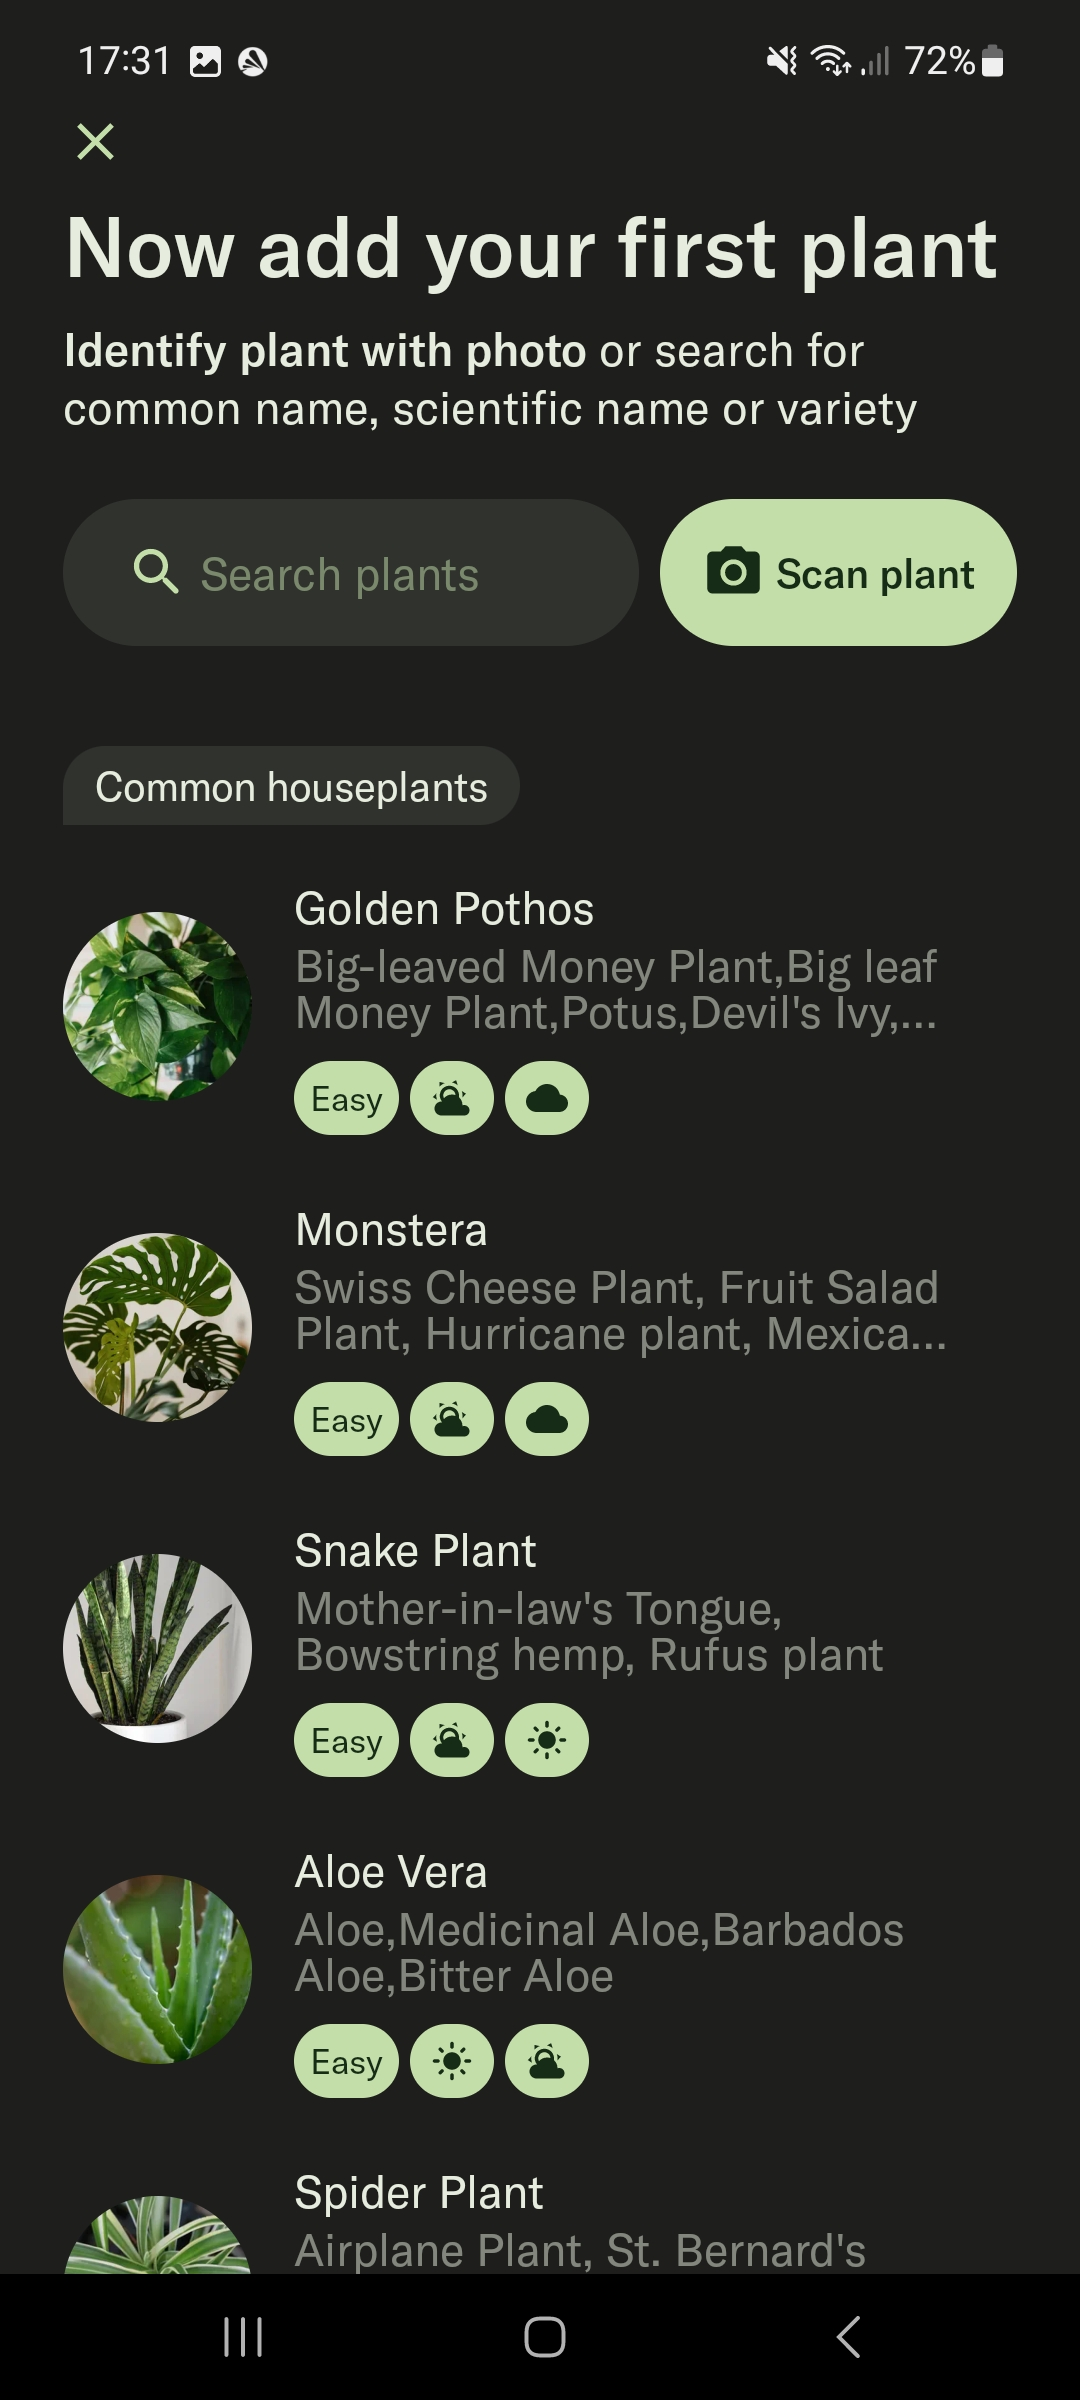
\includegraphics[width=0.3\textwidth]{img/planta.jpg}
	\hspace{0.05\textwidth} 
	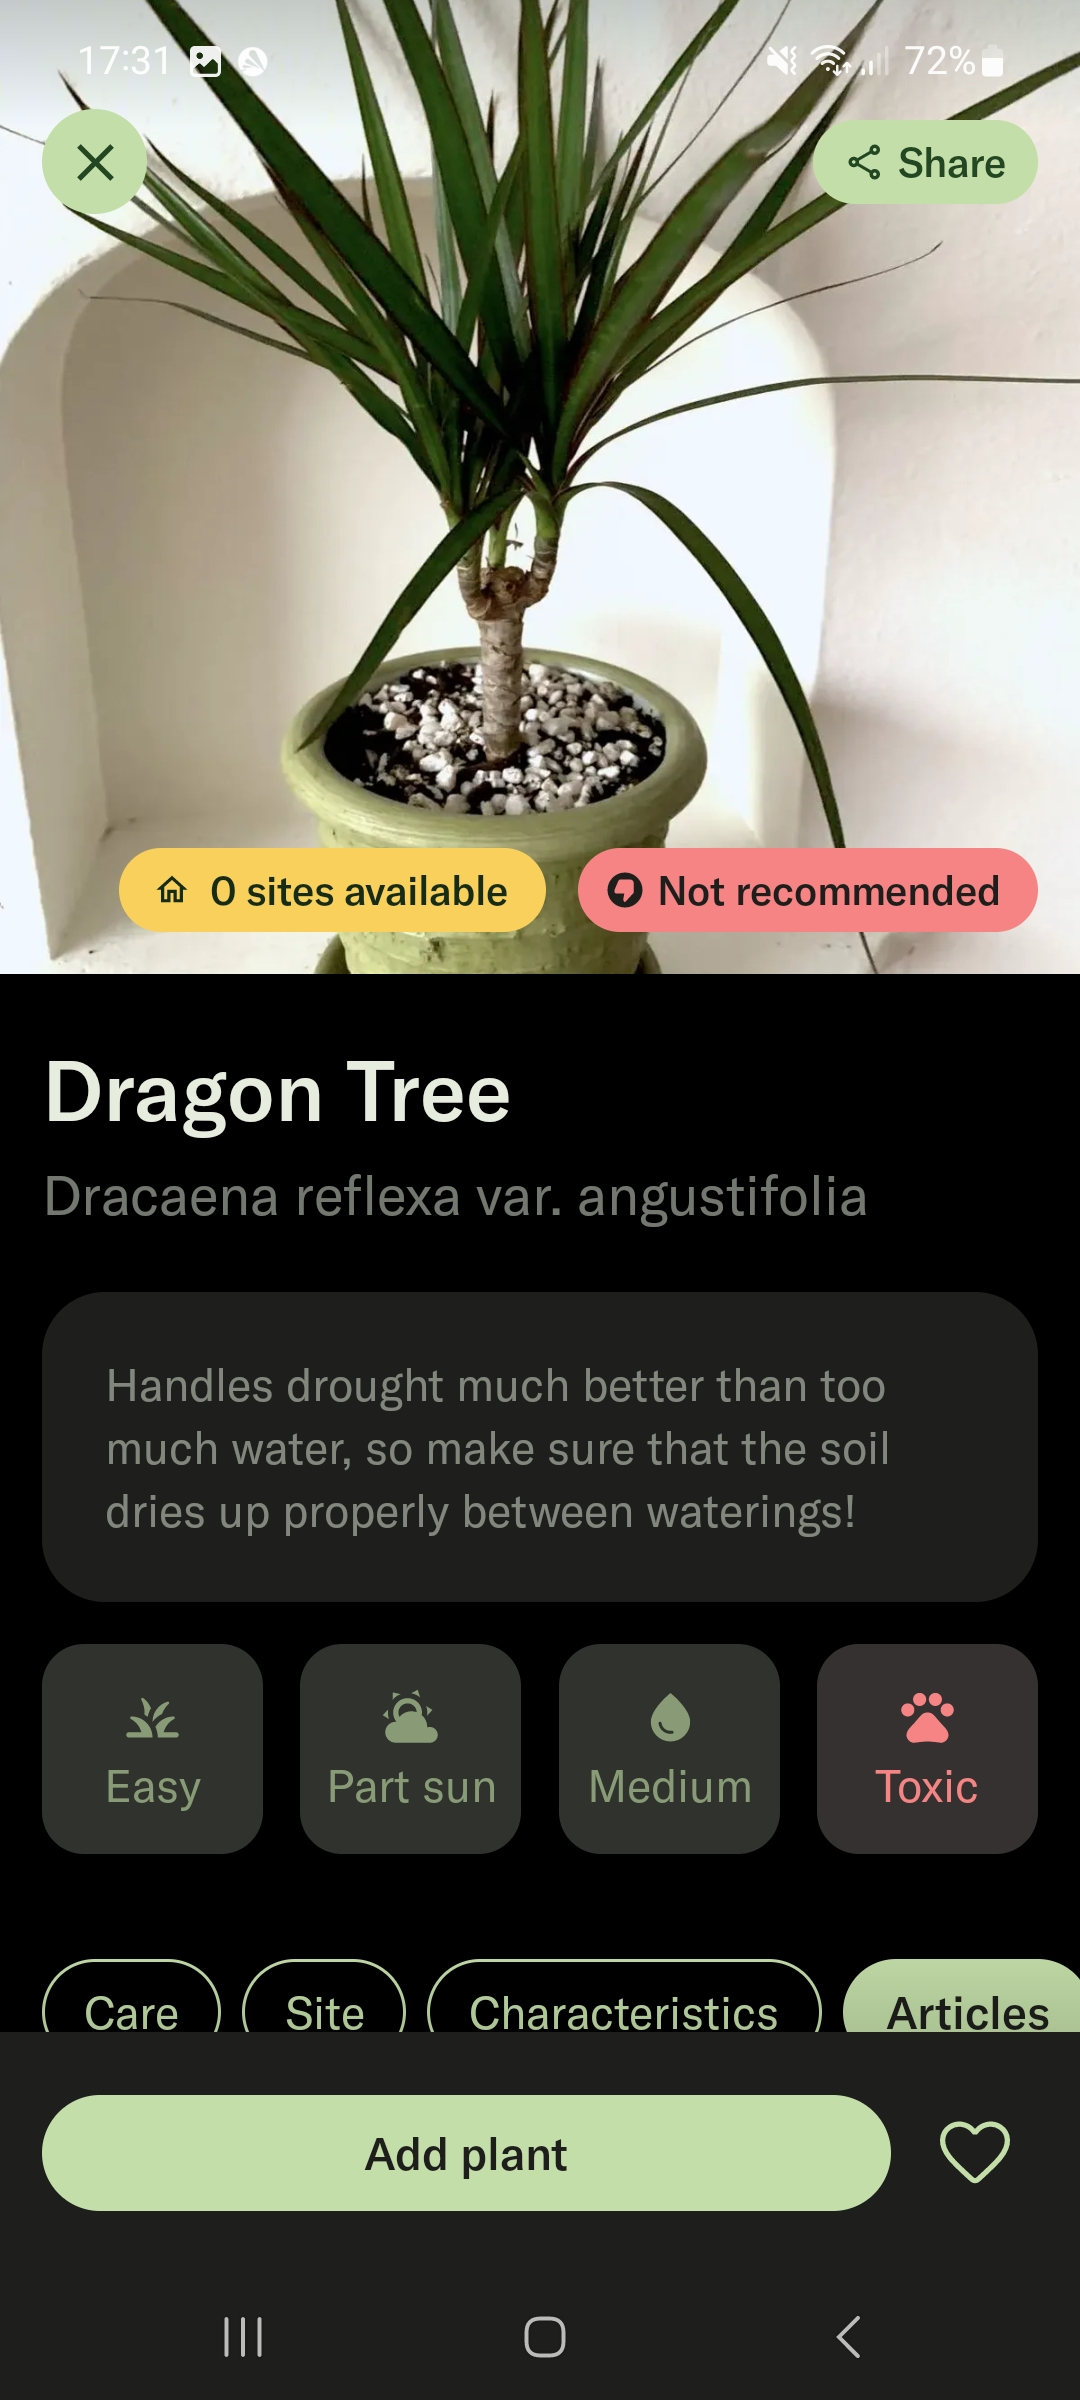
\includegraphics[width=0.3\textwidth]{img/planta2.jpg}
	\caption{Przykładowe zrzuty ekranu z aplikacji Planta.}
	\label{fig:plantazdjecia}
\end{figure}
\subsubsection{Agrio - Plant diagnosis app}
Aplikacja skierowana do miłośników roślin. Pozwala na zrobienie serii zdjęć chorej rośliny, przekazanie jej aplikacji, któa następnie zadaje krótka serie pytań i na podstawie zdjeć oraz informacji z kwestionariusza, dokonuje diagnozy, jednak rozpoznaje tylko chorobę i rodzinę rośliny - nie poda informacji szczegółowych na temat gatunku ze zdjęcia. Aplikacja pozwala także, za dodatkową opłatą, na skonsultowanie się z ekspertem. Prócz funkcji diagnozy, posiada także system czat AI, gdzie użytkownik może zadawać różne pytania na temat flory. Aplikacja posiada także funkcje społecznościowe\cite{Agrio}.
\begin{figure}[H]
	\centering
	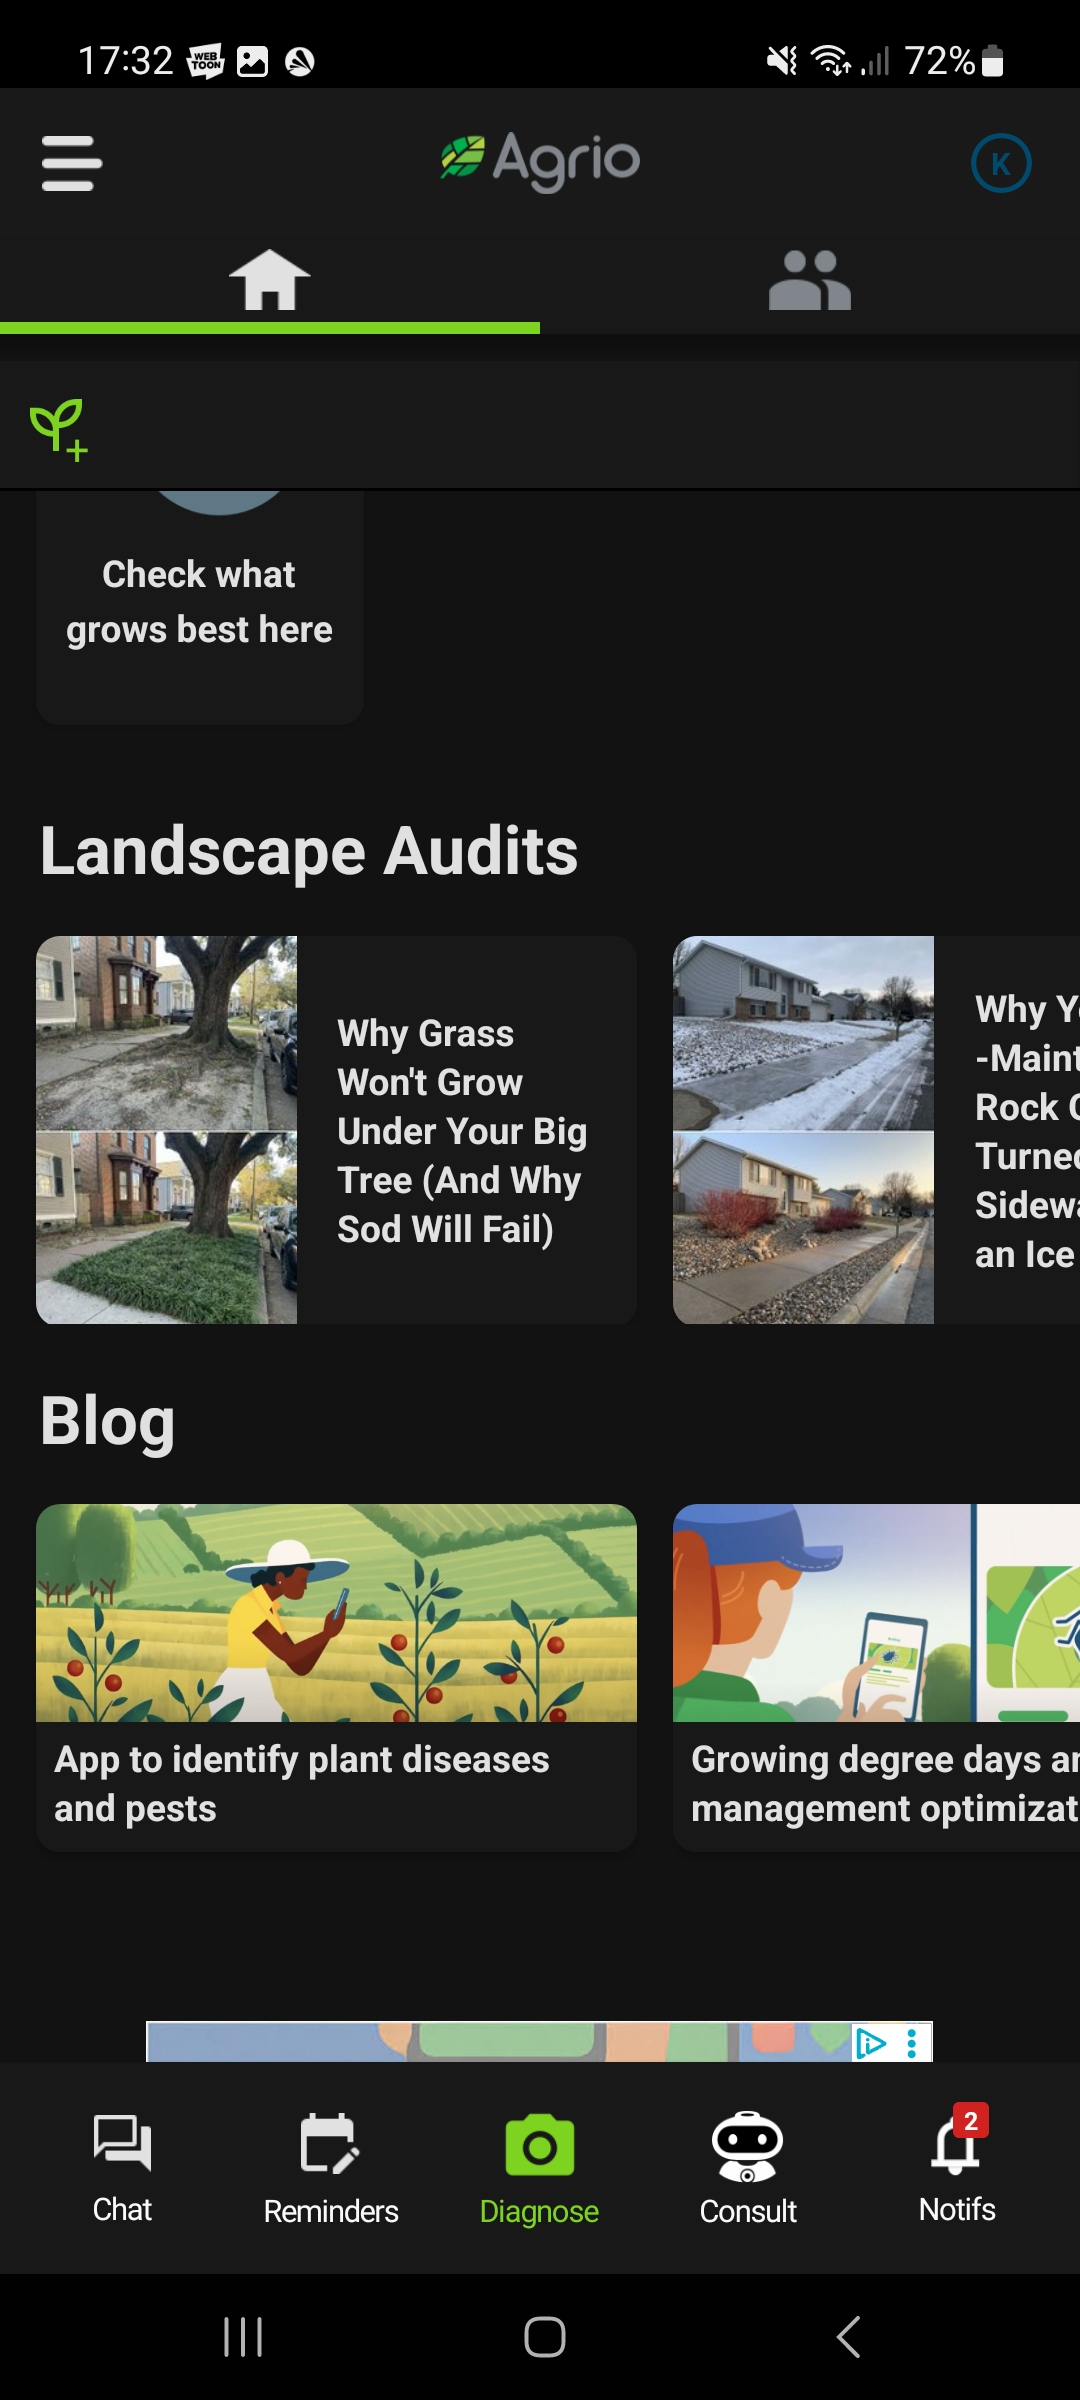
\includegraphics[width=0.3\textwidth]{img/agrio1.jpg}
	\hspace{0.05\textwidth} 
	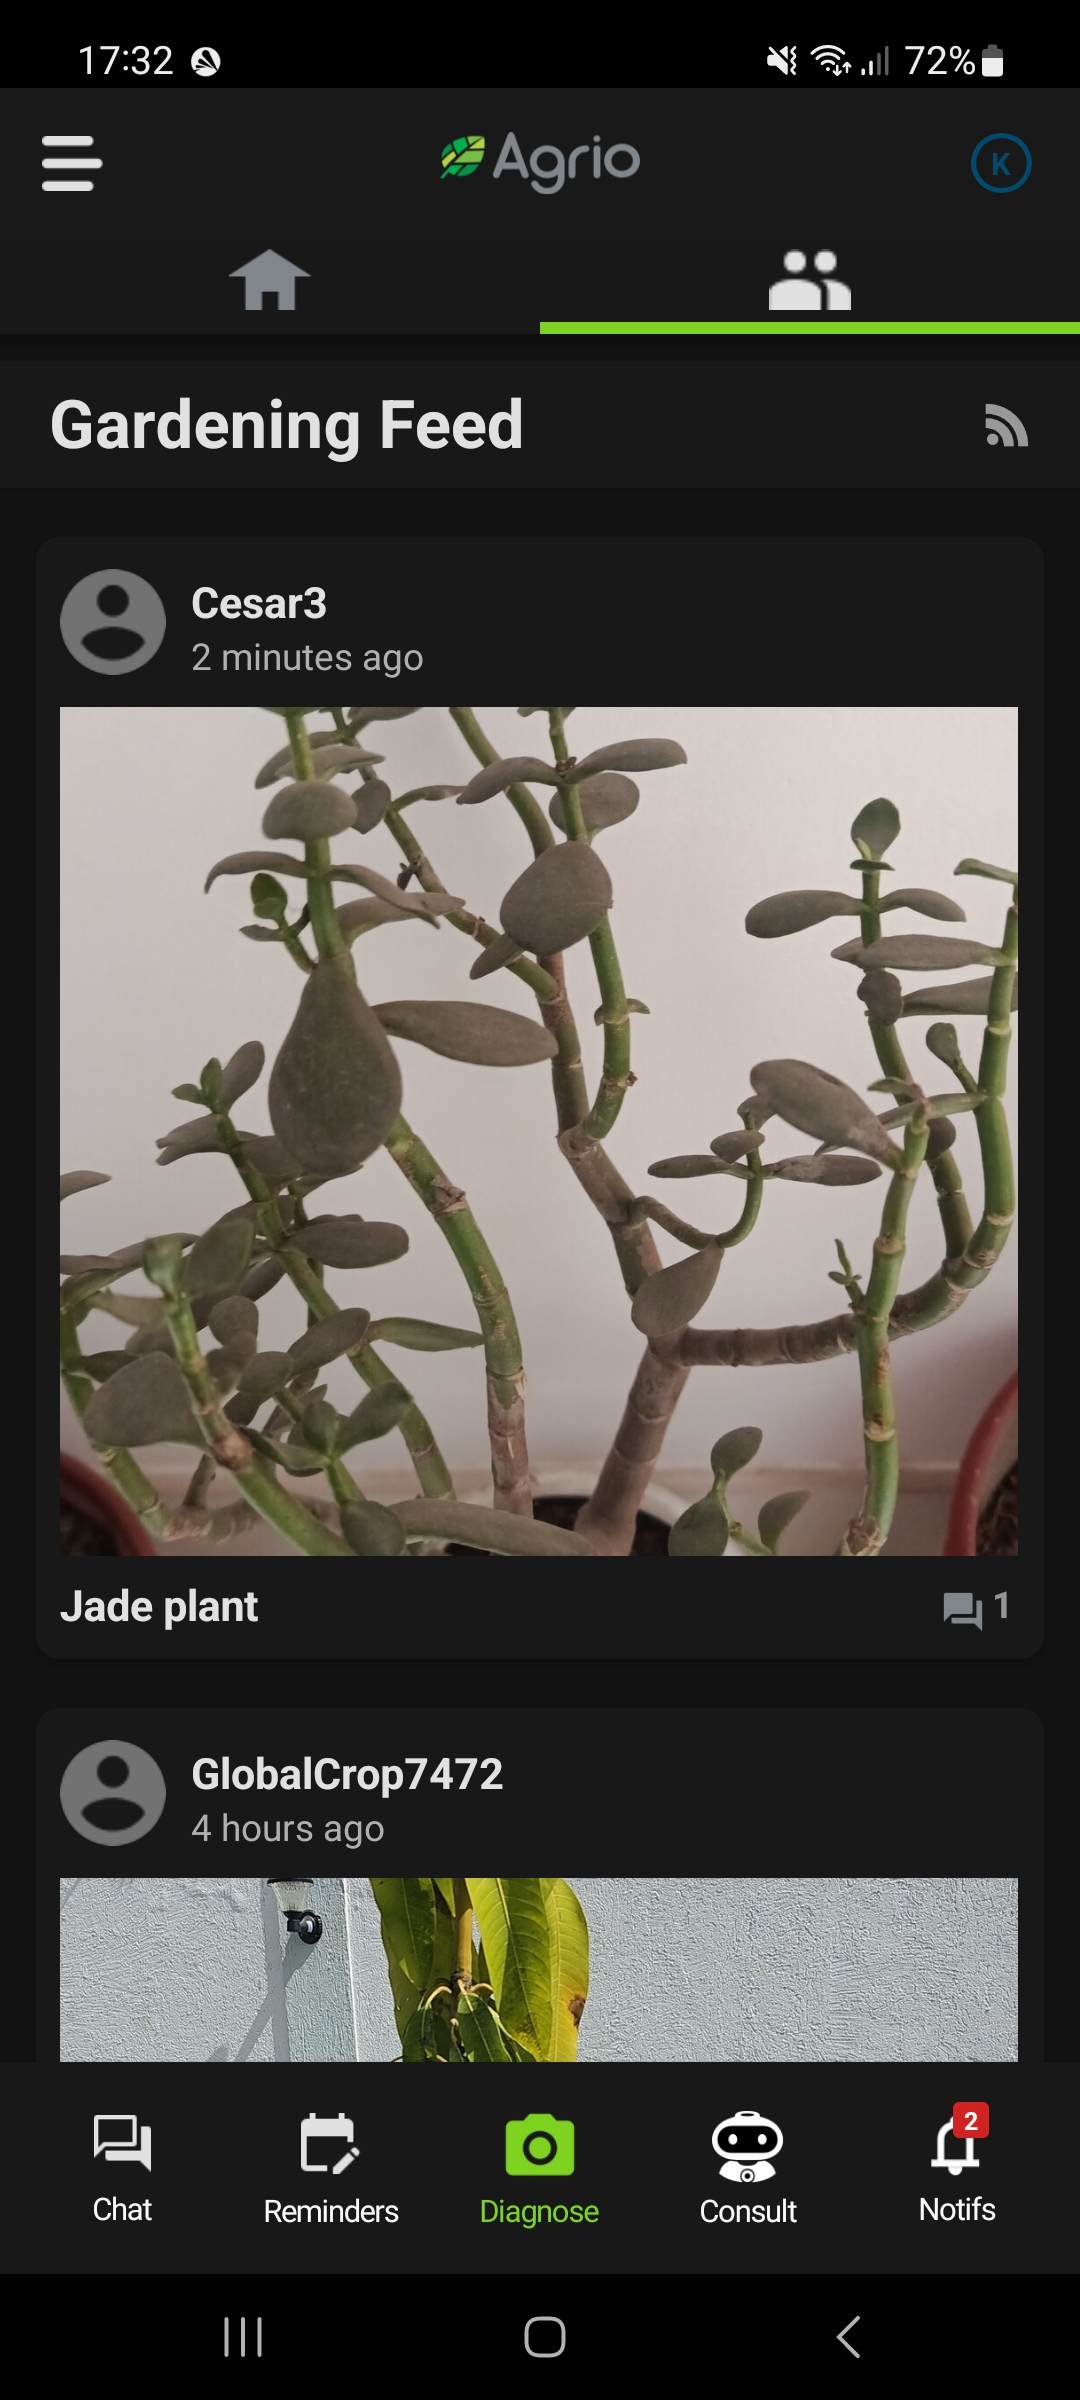
\includegraphics[width=0.3\textwidth]{img/agrio2.jpg}
	\caption{Przykładowe zrzuty ekranu z aplikacji Agrio.}
	\label{fig:agriozdjecia}
\end{figure}
\subsubsection{PlantNet Plant Identification}
Aplikacja pozwala na identyfikacje roślin na podstawie kilku metryk, np. na podstawie zdjęcia liści, kwiatu, czy ogólnego habitatu. Przedstawia także inne, prawdopdoobne gatunki pasujące do dostarczonych danych. Posiada także atas roślin, gdzie każdy gatunek z bazy ma przypisaną nazwę w wybranym z dostępnych języków, nazwę łacińską, zdjęcia, linki do źródeł informacji takich jak np. Wikipedia, oraz status gatunku w czerwonej księdze IUCN\cite{PlantNet}.
\begin{figure}[H]
	\centering
	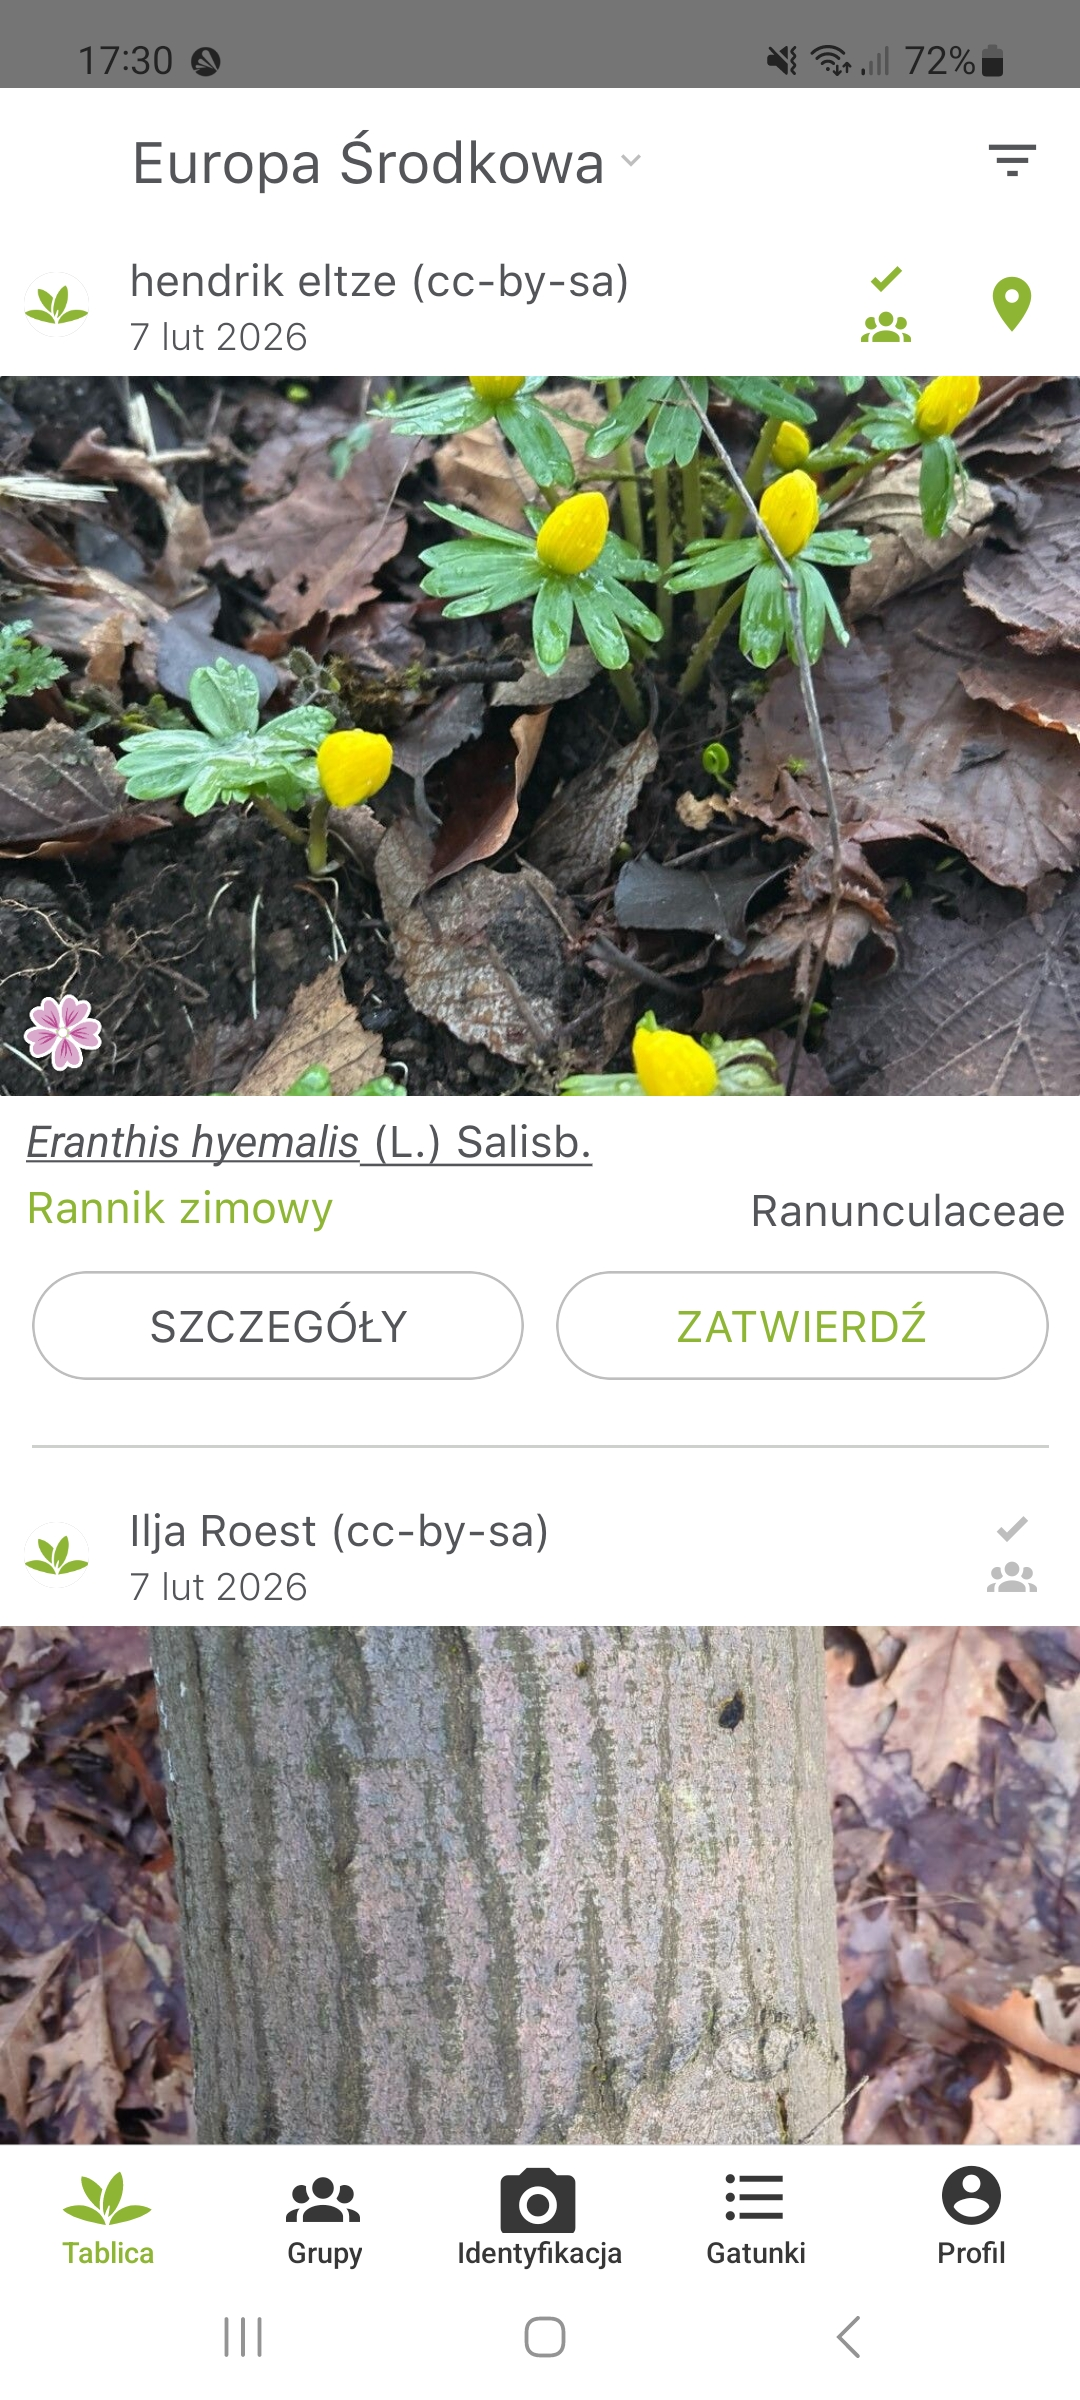
\includegraphics[width=0.3\textwidth]{img/plantnet1.jpg}
	\hspace{0.05\textwidth} 
	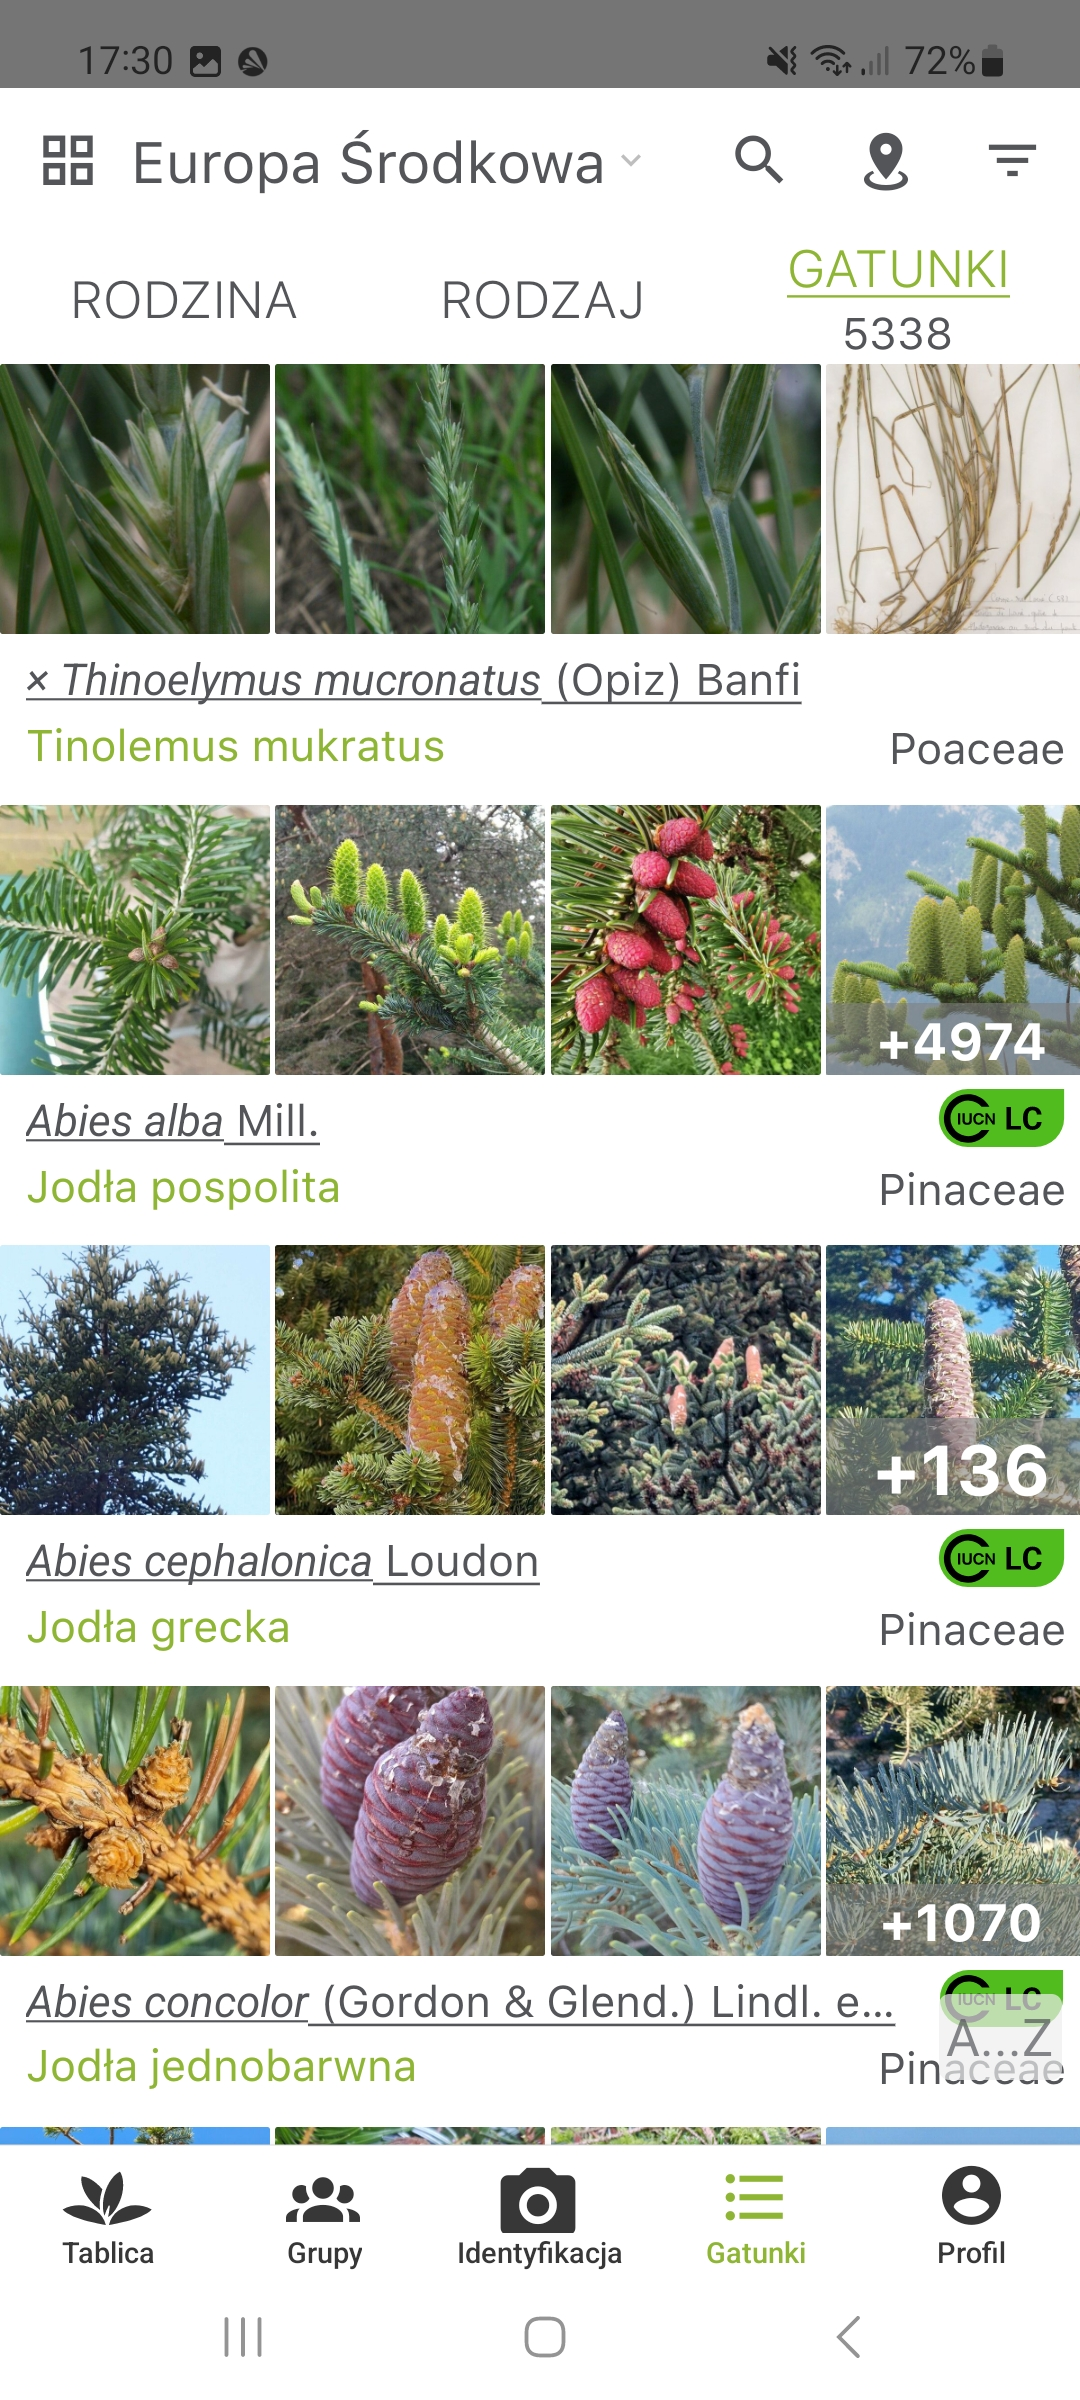
\includegraphics[width=0.3\textwidth]{img/plantnet2.jpg}
	\hspace{0.05\textwidth} 
	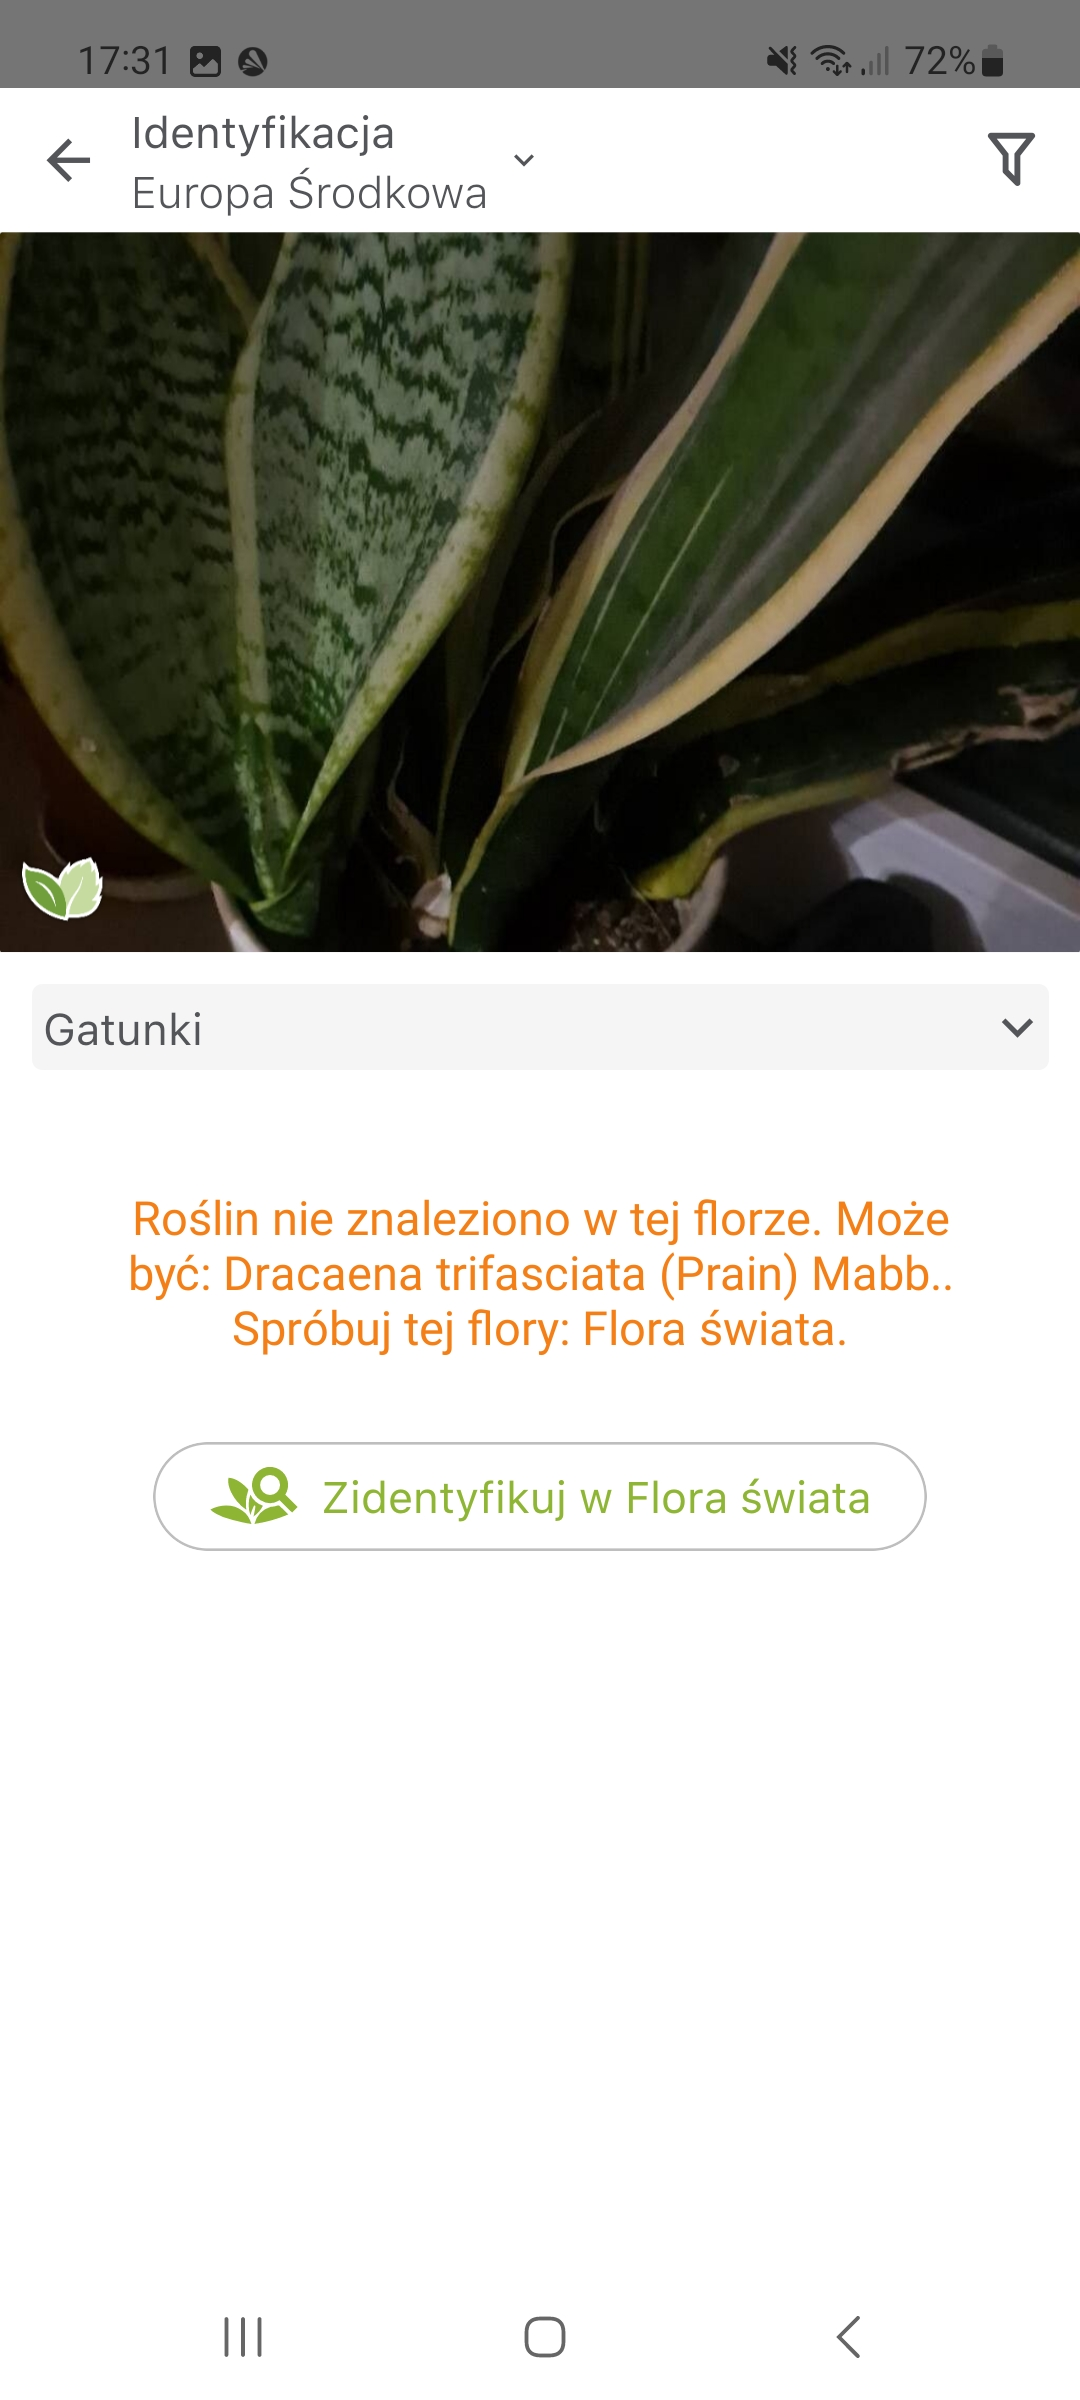
\includegraphics[width=0.3\textwidth]{img/plantnet3.jpg}
	\caption{Przykładowe zrzuty ekranu z aplikacji.}
	\label{fig:agriozdjecia}
\end{figure}


\clearpage